\chapter{FlipIt game with virus propagation}
\label{cha:9}
%\documentclass[10pt]{article}
%\begin{document}

%%%%%%%%%%%%%%%%%%%%%%%%%%%%%%%%%%%%%%%%%%%%%%%%%%%%%%%%%%
%%%%%			Introduction Chapter 1				%%%%%%
%%%%%												%%%%%%
%%%%%												%%%%%%
%%%%%%%%%%%%%%%%%%%%%%%%%%%%%%%%%%%%%%%%%%%%%%%%%%%%%%%%%%

\section{Introduction}

\section{FlipIt game with virus propagation}

Motivatie voor het veranderen van FLipIt naar een FlipIt met viruspropagatie:

\section{Explaining difference between FlipIt with and without virus propagation}

In chapter 2 the FlipIt game was explained.  This chapter starts from the specific case of a non-adaptive continuous FlipIt game where both players play a periodic strategy with a random phase. This choice is motivated by the assumption that in the practical situation of most organisations, the defence strategy is to periodically defend the network. This corresponds to a periodic defender strategy. \todo{bedrijven hebben niet het geld en de mankracht om zich daar mee bezig te houden en dan is periodisch verdedigen het handigste, bedrijven willen alles zo efficient en met de minste kost doen} To simplify the analysis in a first time, a periodic attacker strategy is assumed as well. Further research can investigate the effect of relaxing this assumption.\\


A FlipIt game consists of a single resource. To represent the security problem, the game now defines its single resource as a computer network with multiple
nodes. One of the players, the defender, will try to defend his network. The defender
will do this by flipping all the nodes of the network (i.e. the entire resource) in every move he plays. The
attacker, the other player, will try to infect all the nodes in the network. The attacker
will do this by flipping the node in the graph that can infect all the nodes in the
shortest time possible. After dropping a virus on the first node, it takes a while for the virus to infect the entire network. However, since the original FlipIt game works with a single resource that is always flipped entirely, the assumption is made that the attacker is considered to have gained the control over the resource only when all the nodes of the network have been infected, i.e. the entire resource has been flipped.

After dropping a virus on the first resource, it takes a while for the virus to infect
the entire network. The time that it takes for the virus to infect every node will be
denoted as parameter d. If we want to measure how long it takes for the virus to
infect all the nodes in the network, we have to calculate the shortest path from the
first infected node to the farthest node. This can be measured by a method that we
will explain in section []. Assume that an attacker attacks at time t, then only at time t + d he gains control over the entire network. If the defender flips the network before the period d has elapsed (so, somewhere between t and t+ d), then the attacker will never gain control over the entire network. Using this parameter d, a FlipIt game with virus propagation
can be modelled. 

%------------------------------------------------%
%            Intro Game Theory 					 %
%------------------------------------------------%
\subsection{Actions of the attacker}
A virus has different kind of ways of making his way through a company network. We will describe the different ways of how the virus can propagate. For start we will say that the virus or worm will be dropped on Node i and that it has k numbers of neighbours. 
\begin{enumerate}
\item Node i is infected and will spread the virus or worm to every k neighbours and will stop infecting the neighbours in the next step
\item Node i is infected and will spread the virus or worm to every k neighbours and will keep on spreading the virus to the same neighbours in every next step
\item Node i is infected and will spread the virus to only one of the k neighbours and will stop infecting another neighbour in the next step
\item Node i is infected and will spread the virus to only one of the k neighbours and in the next step it will infect another one of the k neighbours 
\end{enumerate}

In the game that will be modelled in the paper we will use the settings of the first spreading method. We will not use method 2 because this kind of propagation will float the network. Because we use the settings of a mail system and contact in a mailing list the method of 3 and 4 are not used. \\
In the first method the node that has been infected can be again infected. If one of the neighbours infects the node again the node will infect his neighbours again. By using this spreading method we have three distinct states in which a node can be situated. An \textit{infected state}, a \textit{clean state} and a \textit{spreading state}. An infected state means that the node is infected and will not spread the virus to its neighbours, a clean state means that the node is not infected on that moment and a spreading state means that the node is infected and that it will spread the virus or worm to its neighbours in the next step.
We can argument this kind of propagation through a mail worm. \todo{voorbeeld geven van zo een worm}
%Another propagation method is that the virus works as a token. It will propagate to only one neighbour and continue to spread. 

The Attacker itself has two different ways of attacking the company network. It will only infected one node of the network and will wait for the virus to spread itself through the network. We will model two ways of attacks of an Attacker:
\begin{enumerate}
\item The attacker drops the virus on a random node on the network
\item The attacker drops the virus on a targeted node on the network
\end{enumerate}
The attacker in this game will put a virus or worm on one of the nodes in the network. (This will happen at random.) The attacker does not know on which node the virus will be dropped. We will use this randomness because \todo{feit uit security rapport symantec} most viruses are spread via a usb stick or a shared resource. If we use this spreading method where we have a targeted attack the attacker will have more information about the network. \\

The attacker can choose at which rate it will drop a virus on one of the nodes on the network. The cost of dropping a virus will be the same. It will not increase. If it will increase this means that the attacker will eventually drop out of the game because it becomes to expensive.\\
The attacker is in control over the game if it manages to infect a subset of all the resources of the company network.


\subsection{Actions of the defender}
The attacker wants to protect all the nodes of his network. It can do so by getting back control over the resources. We will assume that the defender of the network has knowledge over his own network. Which is convenient in the real world because a company has to know how his infrastructure looks like.\\

The defender has two possible ways of defending its network:
\begin{enumerate}
\item The defender flips all the nodes of his network
\item The defender will flip a subset of the nodes of his network
\end{enumerate}

The cost of flipping all the nods of the network will be greater than the cost of flipping a subset of nodes. We make this assumption because otherwise it will be beneficial for the defender to always flip all the nodes in the network.\\

We will also make the assumption that as a defender flips a node the node can get infected again. A flip will not be  correlated to a patch but to a clean-up. \todo{waarom geen patch, wormen kunnen veranderen gaandeweg}
\todo{andere mogelijkheid:} Another setting of the game can be that the flip of the defender is equal to a patch and that the resource cannot be infected any more. But with this case we deviate from the flipIt game, because the attacker cannot flip the resource any more. Unless we work with different virusses every time the attacker flips. We start with the less complex game of flipping is equal to a clean-up.


\section{Formal definition Game}

In this section we provide a formal definition of the game and the notation that we will use throughout the paper. 


\section*{Playing periodically with virus propagation}

This chapter explains how to model a FlipIt game with a virus propagation that infects a network. The first section explains the difference between a normal FlipIt game and a FlipIt game with virus propagation. The next section derives a formula to calculate the benefit for a FlipIt game with a virus propagation. In the last section we calculate the Nash equilibrium for the benefit formula.




\section{Benefit for a periodic FlipIt game with virus propagation}
We start by formalizing the non-adaptive continuous basic FlipIt game where players use a periodic strategy with a random phase. Next we split the formalisation for the benefit formula for a FlipIt game with virus propagation in two cases. First the benefit formula is derived for the basis case and then it is calculated for the case with a virus propagation. One case is where the defender plays at least as fast as the attacker, the other case is where the attacker plays at least as fast as the defender. This subdivision is also used in the FlipIt paper. \\

 A Periodic strategy is a non-adaptive renewal strategy where the time intervals between consecutive moves are a fixed period, denoted by $\delta$. Moreover it has a random phase, that is chosen uniformly and random in the interval $[0,\delta]$ for the first move. The average rate of play of a player is denoted by $\alpha_{i} = \dfrac{1}{\delta_{i}}$. \\
~~\\


\subsection*{\textbf{Case 1:} $\delta_{D} \leq \delta_{A} $ (The defender plays at least as fast as the attacker.) }

Let $r = \dfrac{\delta_{D}}{ \delta_{A} }$. The intervals between two consecutive defender's moves have length $\delta_{D}$. Consider a given defender move interval. The probability over the attacker's phase selection that the attacker moves in this interval is r. Given that the attacker moves within the interval, he moves exactly once within the interval (since $\delta_{D} \leq \delta_{A} $) and his move is distributed uniformly at random. \\

The expected period of attacker control within the interval would be r/2, without considering the delay by a virus. Therefore the benefit without this virus can be expressed as follows:
\begin{equation}\label{first}
\beta_{D}(\alpha_{D},\alpha_{A}) =1 -  \dfrac {r} {2} - k_{D} \alpha_{D} = 1 - \dfrac {\delta_{D}} {2\delta_{A}} - k_{D} \alpha_{D} 
\end{equation}
\begin{equation}\label{first}
\beta_{A}(\alpha_{D},\alpha_{A}) =\dfrac {r} {2} - k_{A} \alpha_{A} = \dfrac {\delta_{D}} {2\delta_{A}} - k_{A} \alpha_{A}  
\end{equation}\\

However, because of the delay caused by a virus, the maximal time of control is reduced to $\delta_{D}-d$. There is a probability of \textit{r} that the attacker will move in the interval of the defender. The attacker has to play soon enough to gain control, meaning that the attacker has to play during the period of $\delta_{D}-d$ during the interval of the defender. There is $\dfrac{\delta_{D}-d}{\delta_{D}}$ probability that the attacker will move soon enough which gives the attacker a gain of $\dfrac{\delta_{D}-d}{2}$. If the attacker moves after the period of $\delta_{D}-d$, the gain of the attacker will be zero. The average gain rate of the attacker can be expressed as follows if we look at one interval of the defender:
\begin{equation}\label{first}
\gamma_{A}(\alpha_{D},\alpha_{A}) = \dfrac {1}{\delta_{D}} [ \dfrac{\delta_{D}}{\delta_{A}} \cdot \dfrac{\delta_{D}-d}{\delta_{D}} \cdot \dfrac{\delta_{D}-d}{2} + \dfrac{\delta_{D}}{\delta_{A}} \cdot \dfrac{d}{\delta_{D}} \cdot 0 ]
\end{equation}

To complete the formula to derive the benefit function, the cost of moving is added. In the second formula we can see the formula of the original FlipIt game.
\begin{equation}\label{first}
\beta_{A}(\alpha_{D},\alpha_{A}) = \dfrac { (\delta_{D}-d) ^{2}} {2 \cdot \delta_{D}  \delta_{A}} - k_{A} \alpha_{A}
\end{equation}
\begin{equation}\label{first}
\beta_{A}(\alpha_{D},\alpha_{A}) = \dfrac { \delta_{D}} {2 \cdot \delta_{A}} - k_{A} \alpha_{A} + \dfrac{d}{\delta_{A}} + \dfrac{d^{2}}{2 \cdot \delta_{A} \delta_{D}}
\end{equation}
 
 The benefit of the defender is expressed as follows:
 \begin{equation}\label{first}
\beta_{D}(\alpha_{D},\alpha_{A}) = 1 - \dfrac { (\delta_{D}-d) ^{2}} {2 \cdot \delta_{D}  \delta_{A}} - k_{D} \alpha_{D}
\end{equation}
~~\\





\subsection*{\textbf{Case 2:} $\delta_{A} \leq \delta_{D} $ (The attacker plays at least as fast as the defender.) }

First let $r = \dfrac{\delta_{D}}{ \delta_{A} }$. The intervals between two consecutive attacker's moves have length $\delta_{A}$. Consider a given attackers move interval. The probability over the attacker's phase selection that the defender moves in this interval is $\dfrac{\delta_{D}}{ \delta_{A} } = (1/r)$. Given that the defender moves within the interval, he moves exactly once within the interval (since$\delta_{A} \leq \delta_{D} $) and his move is distributed uniformly at random. \\

A similar analysis as in case 1 for a FlipIt game without virus propagation yields the following benefits:
\begin{equation}\label{first}
\beta_{D}(\alpha_{D},\alpha_{A}) = \dfrac {1} {2r} - k_{D} \alpha_{D} = \dfrac {\delta_{A}} {2\delta_{D}} - k_{D} \alpha_{D} 
\end{equation}
\begin{equation}\label{first}
\beta_{A}(\alpha_{D},\alpha_{A}) =1 - \dfrac {1} {2r} - k_{A} \alpha_{A} = 1- \dfrac {\delta_{A}} {2\delta_{D}} - k_{A} \alpha_{A}  
\end{equation}\\


For the case with a virus we consider two cases, \textbf{Case a} and \textbf{Case b}, to compute the benefit of both players.  \\


\subsubsection*{\textbf{Case a:} $d + \delta_{A} \leq \delta_{D}$}

Let $d + \delta_{A} \leq \delta_{D}$. If $d + \delta_{A}$  is a timespan for the attacker, the defender will never move twice in this timespan.  $\dfrac{delta_{A}}{\delta_{D}}$ the defender will move during the interval of the attacker. When this happens the defender will end with beeing in control at the end of the interval. In the next interval the attacker will move in the beginning but will not gain control after the delay of \textit{d}. This means that if the defender moved in the interval prior to this one, the delay is the minimum gain of the defender. To calculate the gain rate of the defender we don't look at one interval of the defender. We know that if the defender moves within the interval of the defender it will receive a minimum of $\dfrac{\delta_{A}}{2}$ gain. In the next interval the defender will receive a minimum gain of $d$. It is also possible that the defender will move in this interval after the delay, adding a gain of $\dfrac{\delta_{A}}{2}$, but the defender will never play during the delay if in the interval prior to this, the defender already has moved. 

This means that every time the defender plays it will get a benefit of $\dfrac{\delta_{A}}{2}$ and the next interval will always receive a gain of $d$. To derive the benefit formula for the defender we can calculate the probability that the defender will move during an interval of the attacker and multiply it by the gain of the interval plus the gain that it will give to the next interval. 
This yields in the following formula:
\begin{equation}\label{first}
\beta_{D}(\alpha_{D},\alpha_{A}) = \dfrac{\delta{A}}{\delta_{D}} \cdot \dfrac{(d+\dfrac{\delta_{A}}{2})}{\delta_{A}} - k_{D} \alpha_{D} 
\end{equation}
\begin{equation}\label{first}
\beta_{D}(\alpha_{D},\alpha_{A}) = \dfrac{\delta{A}}{2\delta_{D}} + \dfrac{d}{\delta_{D}} - k_{D} \alpha_{D} 
\end{equation}\\

The benefit for the attacker will be as follows:
\begin{equation}\label{first}
\beta_{A}(\alpha_{D},\alpha_{A}) = 1 -\dfrac{\delta{A}}{2\delta_{D}} - \dfrac{d}{\delta_{D}} - k_{A} \alpha_{A} 
\end{equation}\\

\begin{figure}[hbtp]
\caption{Case 2 where d + deltaA < deltaD}
\centering
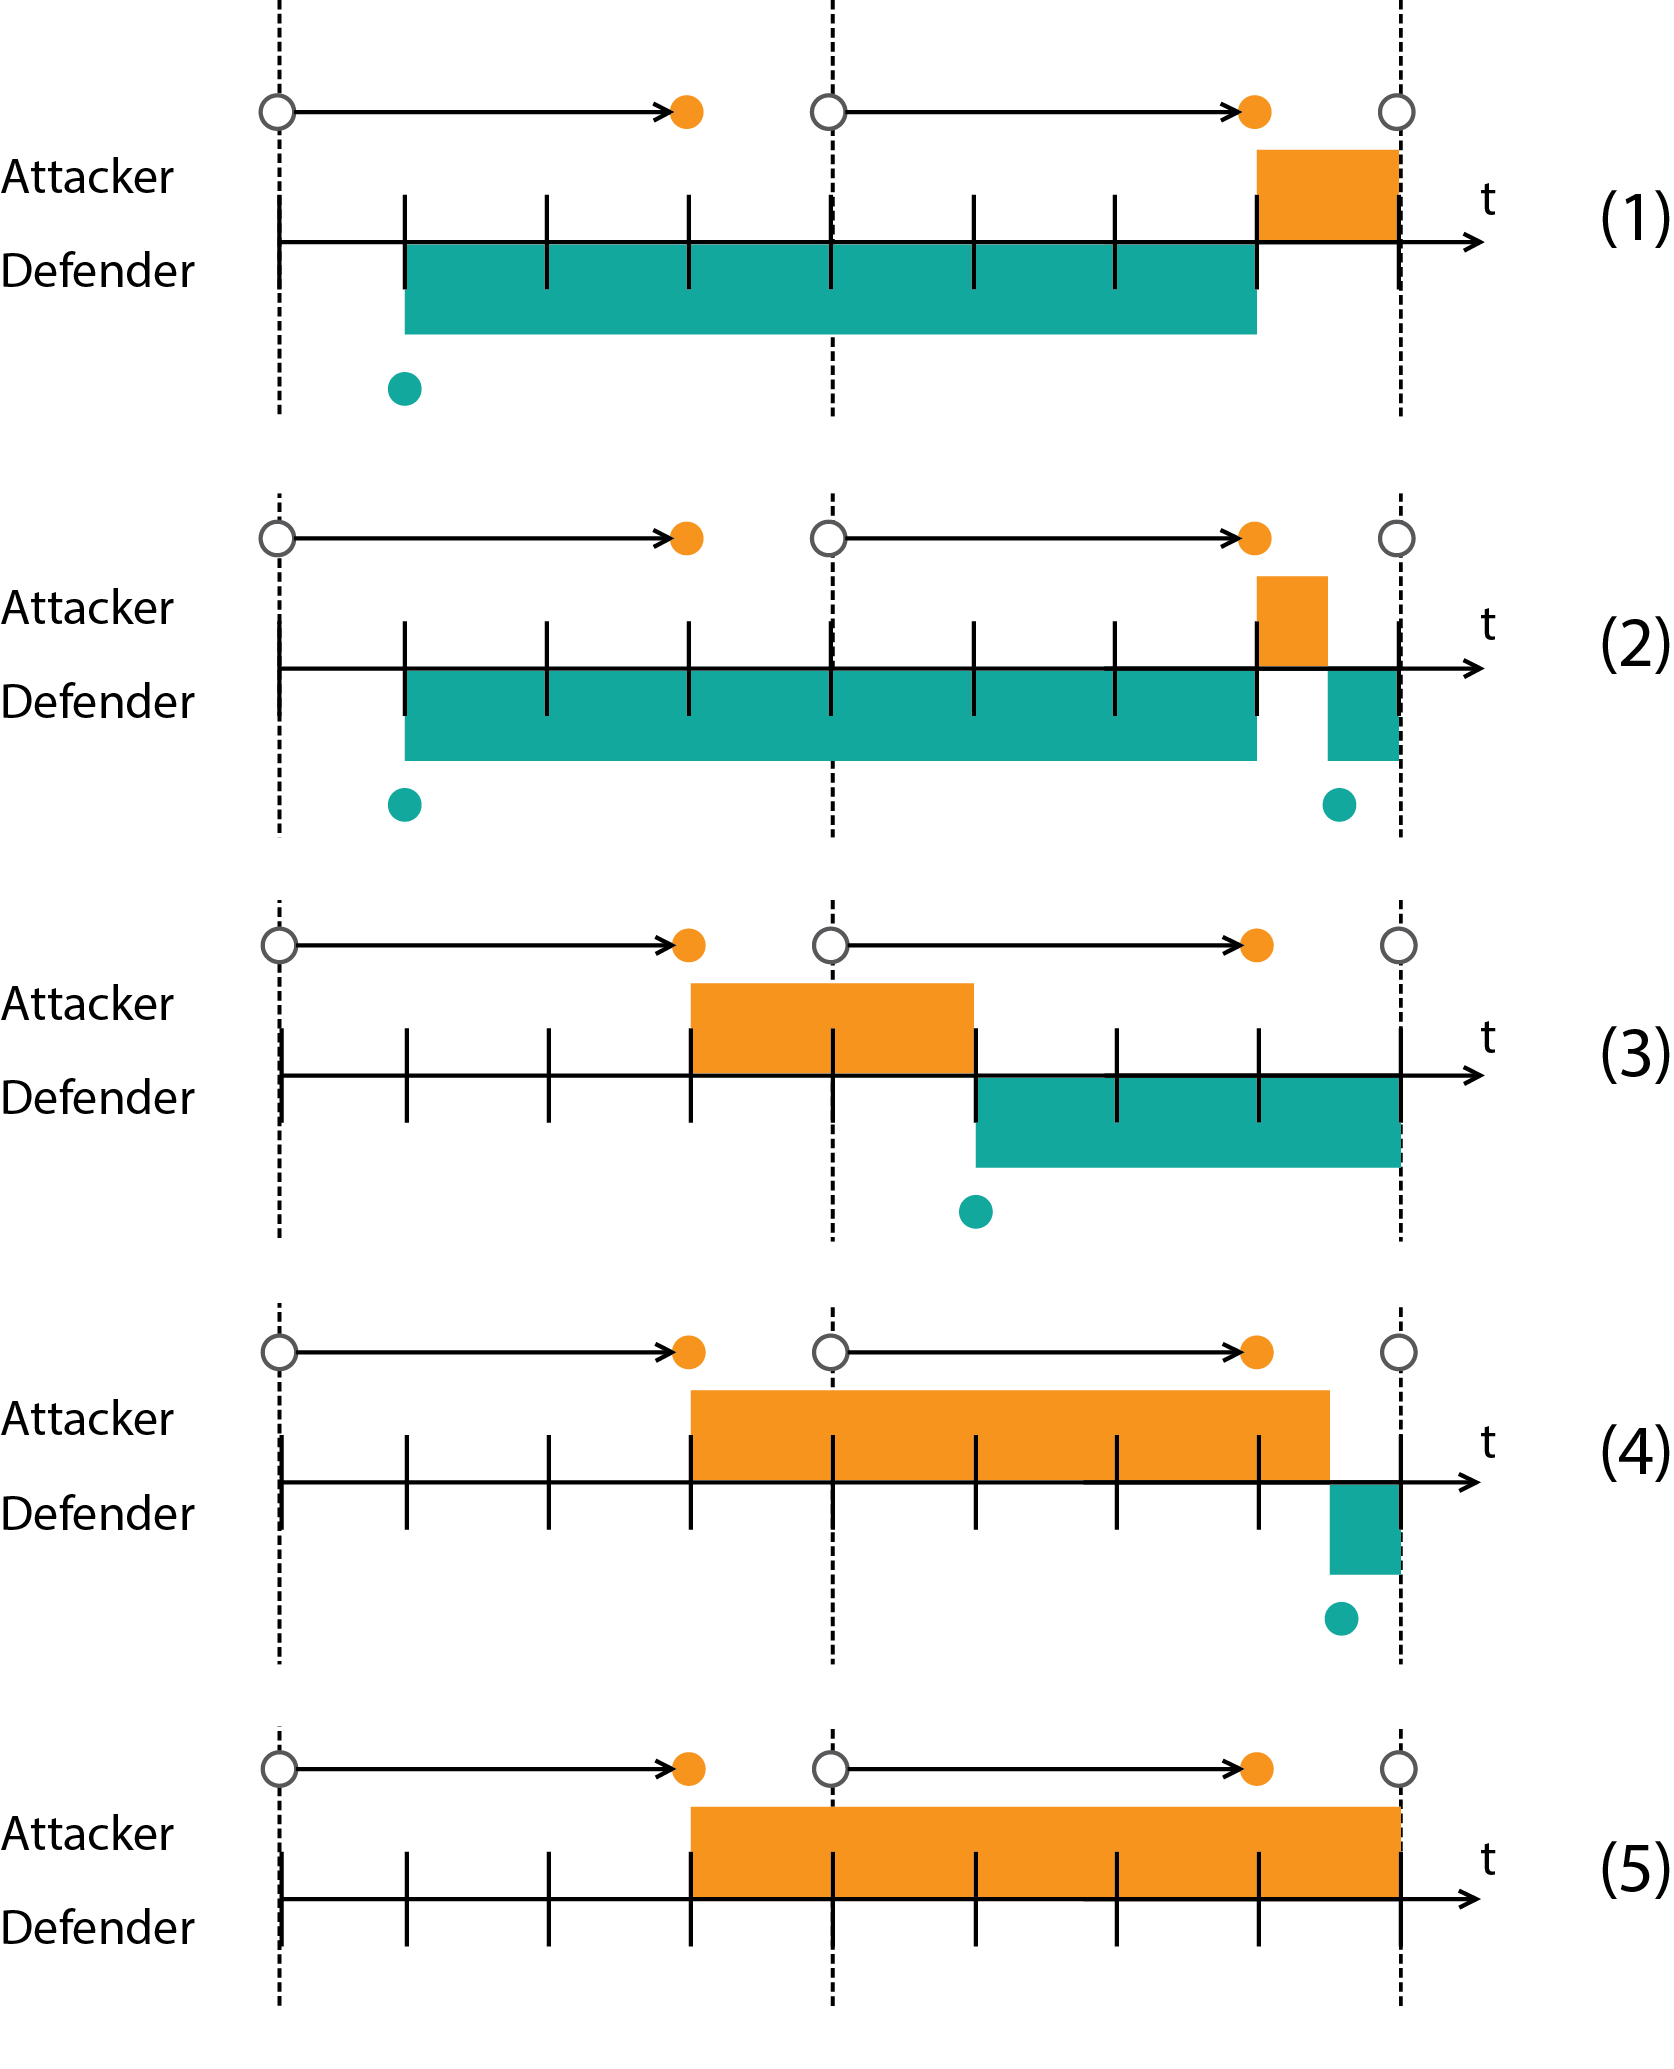
\includegraphics[scale=0.7]{Images/FlipItCase2.png}
\end{figure}


It is crucial that the $d + \delta_{1}$ is not greater than $ \delta_{0}$. If it is greater that means that the defender can move during a delay after an interval of the attacker where the defender already has moved. If we calculate the benefit formula in the same manner, to much gain is added. Namely the overlap during the delay.

\subsubsection*{\textbf{Case b:} $d + \delta_{1} > \delta_{D}$}


\section{Simulation}
%nce the defender has played, it takes 1 time until the attacker plays and the defender loses control again. Therefere, the expected period of attacker control within the interval would be 1/2.1/0, without considering the delay.

%%% Local Variables: 
%%% mode: latex
%%% TeX-master: "thesis"
%%% End: 

%\end{document}
